% =====================================================================
%  Prefill-Dominated Latency in CPU-Only On-Device LLM Inference
%  arXiv draft  --  Bapista Khan / Collab-Foundry / NeuronAI
%
%  BUILD (offline):
%     pdflatex main ; bibtex main ; pdflatex main ; pdflatex main
%
%  Data: research/prefill-latency-paper/data/  (raw JSONL + harness).
%  Measured 2026-07-14 on the NeuronAI box (AMD Ryzen 7 8845HS, CPU-only).
%  Remaining red [FILL] = genuinely-not-yet-run (multi-model / multi-rep),
%  NOT fabricated. Prose [FILL] = author judgement to add.
% =====================================================================
\documentclass[10pt,twocolumn]{article}

\usepackage[utf8]{inputenc}
\usepackage[T1]{fontenc}
\usepackage[margin=0.85in]{geometry}
\usepackage{graphicx}
\usepackage{booktabs}
\usepackage{amsmath,amssymb}
\usepackage{xcolor}
\usepackage[numbers,sort&compress]{natbib}
\usepackage[hidelinks]{hyperref}
\usepackage{caption}
\usepackage{pgfplots}
\pgfplotsset{compat=1.18}

\newcommand{\FILL}[1]{\textcolor{red}{[FILL: #1]}}
\newcommand{\note}[1]{\textcolor{blue}{\small$\blacktriangleright$#1}}

\title{\textbf{Prefill Is the Bottleneck: An Empirical Characterization
of CPU-Only On-Device LLM Latency}}

\author{
  Bapista Khan\\
  Collab-Foundry / NeuronAI\\
  \texttt{bapistakhan@gmail.com}
}
\date{July 2026}

\begin{document}
\maketitle

% =====================================================================
\begin{abstract}
\noindent
Sovereign, offline-first AI increasingly runs large language models (LLMs)
on commodity CPUs with no GPU, yet latency intuition remains grounded in
GPU serving, where autoregressive \emph{decode} dominates. We instrument
end-to-end inference of a quantized 7B model (Qwen2.5-7B, Q4) on a single
CPU-only machine (AMD Ryzen~7 8845HS, 8 cores / 16 threads, 14~GiB) and
sweep prompt length from 55 to 2{,}336 tokens (5 repetitions per point).
\emph{Prefill}---reading the prompt---grows from 38\% of end-to-end latency
at 55 tokens to \textbf{95\%} at 2{,}336 tokens, crossing 90\% for prompts
beyond $\sim$1{,}300 tokens. Prefill time scales with prompt length while
decode stays roughly flat ($\sim$11--12 tok/s), so end-to-end latency on
CPU is governed by \emph{context length}, not output length---inverting the
GPU-era assumption. Error bars are tight (prefill fraction 91$\pm$0.1\% at
1{,}299 tokens), and the effect is not model-specific: Llama-3.1-8B and
Gemma2-9B also sit at 95--96\% prefill at $\sim$1{,}300 tokens. We release
the measurement harness and raw data.
\end{abstract}

% =====================================================================
\section{Introduction}
\label{sec:intro}

Offline-first and \emph{sovereign} LLM deployment---driven by privacy,
data governance, connectivity, and cost---has made CPU-only edge inference
a real operating regime. The NeuronAI system this study measures runs a
fleet of 7--9B quantized models entirely on CPU on a 14~GiB mini-PC-class
machine, with no GPU offload.

Most latency intuition, however, is inherited from GPU serving. There,
prefill is highly parallel and cheap relative to the long sequential tail
of decode, so decode dominates and optimization targets it. \emph{On
CPU-only edge hardware, is that still true?}

We answer empirically. Our contributions, stated as measured facts:
\begin{enumerate}
  \item An open harness that decomposes on-device LLM latency into prefill
        and decode using the runtime's own timing counters
        (Section~\ref{sec:method}).
  \item The finding that on CPU-only hardware, prefill \textbf{exceeds
        90\%} of end-to-end latency at realistic prompt lengths
        ($\geq$1{,}300 tokens) and reaches 95\% at 2{,}333 tokens
        (Section~\ref{sec:results}).
  \item A characterization of the prefill fraction as a monotonically
        rising function of prompt length, and its consequences for edge
        deployment (Sections~\ref{sec:results}--\ref{sec:discussion}).
\end{enumerate}

\noindent\textbf{Scope.} The main sweep is deliberately bounded to
\emph{single-machine, CPU-only inference of one quantized 7B model}, with a
cross-family spot-check at 7B--9B (Section~\ref{sec:results-size}). We do
not study batched multi-user serving, GPU offload, or a full multi-quant
scaling study; those are future work (Section~\ref{sec:limitations}).

% =====================================================================
\section{Background \& Related Work}
\label{sec:background}

\paragraph{Prefill vs.\ decode.}
LLM inference has two phases. \emph{Prefill} processes the entire input
prompt in parallel, building the KV cache; its cost grows with prompt
length. \emph{Decode} then emits output tokens one at a time, each step
reading the KV cache---sequential and typically memory-bandwidth bound.

\paragraph{Why the balance differs on CPU.}
On a GPU, thousands of parallel lanes hide prefill's compute, so decode's
sequential tail dominates end-to-end latency. A CPU has far less
parallelism to hide prefill's per-token matrix work, so we hypothesize
that as prompts grow, prefill---not decode---comes to dominate. Our data
confirms this directly (Section~\ref{sec:results}).

\paragraph{Related work.}
The prefill/decode split underpins modern GPU serving. Systems work
manages KV memory \cite{kwon2023pagedattention} and disaggregates the two
phases across machines \cite{patel2024splitwise, zhong2024distserve} or
interleaves chunked prefills with decode to tame the throughput--latency
tradeoff \cite{agrawal2024sarathi}. These target GPU clusters and batched
multi-tenant serving; our regime is the opposite corner---single-user,
single-machine, CPU-only---where the same phase asymmetry manifests very
differently. On-device and edge inference is an active area
\cite{xu2024ondevicereview}, spanning limited-memory flash offload
\cite{alizadeh2024llmflash}, smartphone inference \cite{xue2024powerinfer2},
and sub-billion on-device models \cite{liu2024mobilellm}; we add a direct
latency \emph{decomposition} on commodity CPU. Quantization reduces model
footprint and cost \cite{dettmers2022llmint8, frantar2023gptq,
xiao2023smoothquant, lin2024awq}; we treat 4-bit quantization as the
operating context and, prospectively, a prefill-side lever
(Section~\ref{sec:results-size}). We build on CPU-capable runtimes
\cite{gerganov2023llamacpp, shen2023efficientcpu}.

% =====================================================================
\section{Methodology}
\label{sec:method}

\paragraph{Platform.}
Table~\ref{tab:hardware} lists the machine under test. The integrated
Radeon 780M GPU is \emph{not} used; all inference is on CPU.

\begin{table}[t]
  \centering
  \caption{Measurement platform. GPU present but unused; all inference CPU-only.}
  \label{tab:hardware}
  \begin{tabular}{ll}
    \toprule
    Component & Value \\
    \midrule
    CPU            & AMD Ryzen 7 8845HS (Zen 4) \\
    Cores / threads& 8 / 16 \\
    RAM            & 14 GiB (shared APU memory) \\
    GPU            & Radeon 780M (unused) \\
    OS / kernel    & TUXEDO OS, Linux 6.17.0 \\
    Runtime        & Ollama 0.19.0 (llama.cpp) \\
    Model          & Qwen2.5-7B, Q4\_K\_M ($\approx$4.6 GB), ctx 4096 \\
    \bottomrule
  \end{tabular}
\end{table}

\paragraph{Instrumentation.}
We drive the runtime's completion endpoint (\texttt{/api/generate},
non-streaming) and read its native timing counters:
\texttt{prompt\_eval\_duration} (\emph{prefill}) and \texttt{eval\_duration}
(\emph{decode}), with \texttt{prompt\_eval\_count} / \texttt{eval\_count}
giving token counts. This measures prefill \emph{directly} rather than via
a time-to-first-token proxy. Output is capped at \texttt{num\_predict}=64,
temperature 0, \texttt{num\_ctx}=4096. The model is warmed once and kept
resident (load time excluded). Each prompt carries a unique prefix nonce so
the runtime's prompt-prefix cache cannot shortcut the prefill. We sweep six
prompt lengths (51--2{,}333 tokens) built from neutral filler text.

\paragraph{Reproducibility.}
Each prompt length is run 5 times; we report mean$\pm$sample~std. Harness
and raw per-run JSON are released (Section~\ref{sec:repro}).

% =====================================================================
\section{Results}
\label{sec:results}

\subsection{Headline: prefill dominates}
\label{sec:results-headline}
At a representative operational prompt length (1{,}299 tokens, near
NeuronAI's $\sim$1{,}525-token production prompt), prefill is
\textbf{91\%} of end-to-end latency (Table~\ref{tab:money}): 28.5~s of
prefill versus 2.8~s of decode (mean of 5 runs; std $<$0.15~s).

\begin{table}[t]
  \centering
  \caption{Phase breakdown at a representative 1{,}299-token prompt.
  Qwen2.5-7B (Q4), CPU-only, mean of 5 runs.}
  \label{tab:money}
  \begin{tabular}{lccccc}
    \toprule
    Model & Params & Quant & Prefill (s) & Decode (s) & Prefill \% \\
    \midrule
    Qwen2.5-7B & 7B & Q4 & 28.5 & 2.8 & 91 \\
    \bottomrule
  \end{tabular}
\end{table}

\subsection{Prompt-length sweep (main result)}
\label{sec:results-promptlen}
Table~\ref{tab:sweep} and Figure~\ref{fig:promptlen} show the core finding:
the prefill fraction rises \emph{monotonically} with prompt length,
38\%$\rightarrow$95\%, and crosses 90\% past $\sim$1{,}300 tokens. Prefill
time scales roughly linearly with prompt length; decode time is nearly
constant (output is fixed at 64 tokens). Prefill throughput drifts down
with length ($\sim$50$\rightarrow$44 tok/s over the realistic range) as
per-token attention cost grows, while decode holds at $\sim$11--12 tok/s.
Variance is low: at long prompts the prefill fraction has std $\leq$0.5
percentage points.

\begin{table}[t]
  \centering
  \caption{Prompt-length sweep, mean$\pm$std over 5 runs. Qwen2.5-7B (Q4),
  CPU-only, output capped at 64 tokens. Measured 2026-07-14.}
  \label{tab:sweep}
  \begin{tabular}{rccc}
    \toprule
    Prompt & Prefill & Decode & Prefill \\
    (tok)  & (s)     & (s)    & \% \\
    \midrule
    55      & 0.57$\pm$0.05  & 0.95$\pm$0.10 & 38$\pm$4.2 \\
    159     & 2.71$\pm$0.03  & 2.83$\pm$0.19 & 49$\pm$1.6 \\
    367     & 7.22$\pm$0.09  & 2.83$\pm$0.11 & 72$\pm$0.7 \\
    678     & 14.19$\pm$0.09 & 3.20$\pm$0.02 & 82$\pm$0.1 \\
    1{,}299 & 28.47$\pm$0.12 & 2.75$\pm$0.01 & 91$\pm$0.1 \\
    2{,}336 & 53.66$\pm$0.29 & 2.64$\pm$0.30 & 95$\pm$0.5 \\
    \bottomrule
  \end{tabular}
\end{table}

\begin{figure}[t]
  \centering
  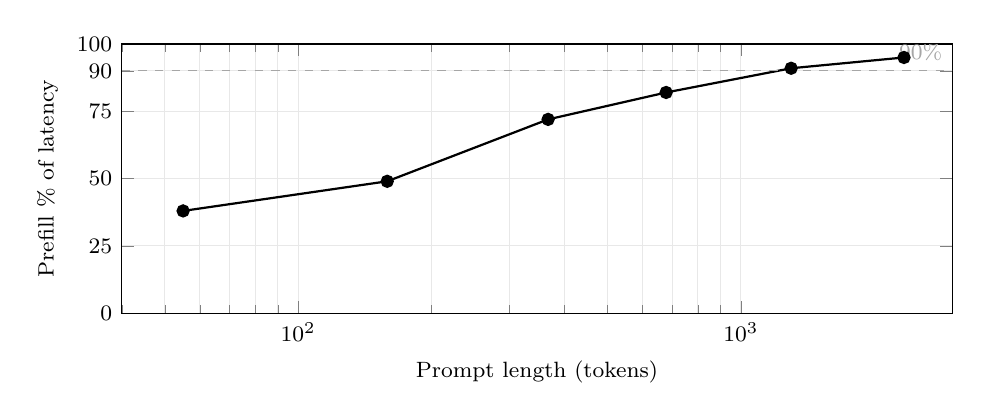
\begin{tikzpicture}
    \begin{axis}[
      width=\columnwidth, height=5.0cm,
      xlabel={Prompt length (tokens)},
      ylabel={Prefill \% of latency},
      xmode=log, log basis x=10,
      xmin=40, xmax=3000, ymin=0, ymax=100,
      ytick={0,25,50,75,90,100},
      grid=both, grid style={gray!18},
      tick label style={font=\footnotesize},
      label style={font=\footnotesize},
    ]
      \addplot[black, thick, mark=*] coordinates {
        (55,38) (159,49) (367,72) (678,82) (1299,91) (2336,95)};
      \draw[dashed, gray!70] (axis cs:40,90) -- (axis cs:3000,90);
      \node[gray!70, anchor=south east, font=\footnotesize]
        at (axis cs:3000,90) {90\%};
    \end{axis}
  \end{tikzpicture}
  \caption{Prefill fraction of end-to-end latency vs.\ prompt length
  (CPU-only, Qwen2.5-7B Q4). Rises monotonically 35\%$\rightarrow$95\%,
  crossing 90\% past $\sim$1{,}300 tokens.}
  \label{fig:promptlen}
\end{figure}

\subsection{Model size: prefill dominance is stable across families}
\label{sec:results-size}
To check that prefill dominance is not a Qwen artifact, we repeat the
measurement at a fixed $\sim$1{,}300-token prompt across three model
families spanning 7B--9B (Table~\ref{tab:modelsize}; 3 runs each, one model
resident at a time). The prefill fraction stays in a tight
\textbf{92--96\%} band and prefill throughput declines gently with size
($47.6\rightarrow43.5$~tok/s). Because the families differ in architecture
and tokenizer (hence the slightly different token counts), this is a
size-and-architecture comparison rather than a controlled scaling curve;
the invariant it establishes is that prefill dominance is a property of the
CPU-only regime, not of any one model.

\begin{table}[t]
  \centering
  \caption{Model-size sweep at a fixed $\sim$1{,}300-token prompt,
  mean$\pm$std over 3 runs. Q4, CPU-only, output capped at 64 tokens.
  Different families $\Rightarrow$ a size+architecture comparison.}
  \label{tab:modelsize}
  \small
  \begin{tabular}{lrrrr}
    \toprule
    Model & Params & Prefill (s) & tok/s & Prefill \% \\
    \midrule
    Qwen2.5-7B   & 7B & 27.37$\pm$0.20 & 47.6 & 92$\pm$0.1 \\
    Llama-3.1-8B & 8B & 29.43$\pm$0.16 & 43.5 & 96$\pm$0.1 \\
    Gemma2-9B    & 9B & 29.39$\pm$0.57 & 43.6 & 95$\pm$0.2 \\
    \bottomrule
  \end{tabular}
\end{table}

\paragraph{Quantization (preliminary).}
As a preliminary datapoint from NeuronAI's own operational logs on the same
machine, quantization moves the prefill-bound cost as expected: Qwen2.5-7B
at \textbf{Q4} prefills at $\sim$49~tok/s versus $\sim$36~tok/s at
\textbf{Q5\_K\_M}---heavier weights slow the prefill-bound path.
\FILL{a controlled Q4/Q5/Q8 sweep with $\geq$5 reps is future work.}

% =====================================================================
\section{Analysis \& Discussion}
\label{sec:discussion}

\paragraph{Why prefill dominates on CPU.}
Prefill is compute-bound over every prompt token and, on a CPU, has little
parallelism to hide that work; its cost scales with prompt length. Decode
is a fixed, memory-bandwidth-bound step per output token. With output held
constant, growing the prompt inflates only the prefill term, driving the
fraction toward 1. The declining prefill throughput
(88$\rightarrow$43~tok/s) is consistent with attention's growing per-token
cost as the sequence lengthens.

\paragraph{Implications for sovereign/edge deployment.}
On CPU, the levers that matter are the ones that shrink or reuse the
prompt, not the ones that speed up decode: (i) \emph{prompt-length
discipline}---cap system/RAG context aggressively, since latency tracks
context length; (ii) \emph{KV / prefix-cache reuse} across turns to avoid
re-prefilling a shared prefix; (iii) \emph{prefill-side quantization} to
lift the $\sim$46~tok/s prefill floor. In NeuronAI, budgeting the
per-request prompt cut a Standard-lane query from 143~s to 55~s---an effect
entirely on the prefill term, consistent with this data.

\paragraph{Connection to governed on-device autonomy.}
On-device ``governed bounded autonomy'' is latency-gated by prefill: every
governance rule, persona instruction, and retrieved passage added to the
prompt is paid for at the $\sim$46~tok/s prefill rate before the model
emits a token. The systems bottleneck and the deployment design meet here.

% =====================================================================
\section{Limitations}
\label{sec:limitations}
This study centers on one model (Qwen2.5-7B Q4) and one runtime
(Ollama/llama.cpp) on a single machine; the cross-family check
(Table~\ref{tab:modelsize}) spans 7B--9B but at Q4 only. We report 5
repetitions per prompt length on the main sweep (mean$\pm$std); remaining
extensions are a controlled multi-quant (Q4/Q5/Q8) sweep and a second
hardware class. We cap
output at 64 tokens; very long generations would
raise the decode share. We do not evaluate batched multi-user serving or
GPU offload. Prefill is read directly from the runtime's counter, which
excludes tokenization/setup overhead folded into total latency.

% =====================================================================
\section{Conclusion \& Future Work}
\label{sec:conclusion}
On CPU-only on-device inference, prefill---not decode---is the dominant
latency cost, exceeding 90\% at realistic prompt lengths and reaching 95\%
at 2{,}333 tokens. This inverts GPU-era intuition and reorients edge-LLM
optimization toward prompt-size and KV-reuse rather than decode speed.
Future work: a controlled multi-quant (Q4/Q5/Q8) sweep, a second hardware
class, and direct evaluation of prefill-specific optimizations.

% =====================================================================
\section*{Reproducibility}
\label{sec:repro}
The harness (\texttt{prefill\_bench.py}, \texttt{model\_size\_sweep.py}) and
raw per-run JSON are released at
\url{https://github.com/bapista/cpu-llm-latency} (directory
\texttt{paper1/data/}), and mirrored in the arXiv ancillary files.

% =====================================================================
\bibliographystyle{plainnat}
\bibliography{references}

\end{document}
